%%%%%%%%%%%%%%%%%%%%%%%%%%%%%%%%%%%%%%%%%%%%%%%%%%%%%%%%%%%%%%%%%%%%%%%%%
\chapter{Planification et architecture}
\label{Chapitre_2}
%%%%%%%%%%%%%%%%%%%%%%%%%%%%%%%%%%%%%%%%%%%%%%%%%%%%%%%%%%%%%%%%%%%%%%%%%%%
\section*{Introduction}
%%%%%%%%%%%%%%%%%%%%%%%%%%%%%%%%%%%%%%%%%%%%%%%%%%%%%%%%%%%%%%%%%%%%%%%%%%%

La planification constitue une étape essentielle dans la mise en œuvre d'un projet. Ainsi, dans ce chapitre, nous allons identifier et analyser \textbf{les différentes parties prenantes} du système. \\Ensuite, nous présenterons \textbf{les besoins fonctionnels} et \textbf{non fonctionnels}, \textbf{les diagrammes de cas d'utilisation}, ainsi que l'organisation du projet en \textbf{sprints} Scrum.
%%%%%%%%%%%%%%%%%%%%%%%%%%%%%%%%%%%%%%%%%%%%%%%%%%%%%%%%%%%%%%%%%%%%%%%%%%%
\section{Identification des acteurs}
\label{section2.1}
%%%%%%%%%%%%%%%%%%%%%%%%%%%%%%%%%%%%%%%%%%%%%%%%%%%%%%%%%%%%%%%%%%%%%%%%%%%

Notre application web implique cinq acteurs principaux :

\begin{itemize}
    \item \textbf{Internaute :} L'internaute peut consulter les actualités, intéragir avec un Chatbot et créer un 
    compte sur la plateforme pour accéder aux système.

    \item \textbf{Utilisateur :} L'utilisateur, qui peut être un client, une agence ou 
    un administrateur, a la possibilité de gérer son profil, consulter les offres et 
    voir son score client, après authentification.

    \item \textbf{Client :} Le client est un utilisateur souhaitant louer un 
    véhicule auprès d'une agence digitale .Suite à l’authentification, il peut consulter ses réservations en cours, 
    contacter une agence et voir son score de fiabilité.

    \item \textbf{Agence :} L'agence est une entreprise de location de véhicules utilisant 
    la plateforme pour gérer son activité.Dès son authentification, elle peut créer et gérer sa vitrine automobile, 
    suivre les réservations et les réclamations, valider ou refuser des demandes et accéder 
    aux statistiques.

    \item \textbf{Administrateur :}Une fois authentifié, l'administrateur supervise l'ensemble de la plateforme 
    pour garantir son bon fonctionnement. Il peut gérer les agences et les utilisateurs, 
    superviser les véhicules, consulter les KPI, détecter les anomalies et configurer les 
    paramètres système.
\end{itemize}

%%%%%%%%%%%%%%%%%%%%%%%%%%%%%%%%%%%%%%%%%%%%%%%%%%%%%%%%%%%%%%%%%%%%%%%%%%%
\section{Diagramme de contexte statique}
\label{section2.2}
%%%%%%%%%%%%%%%%%%%%%%%%%%%%%%%%%%%%%%%%%%%%%%%%%%%%%%%%%%%%%%%%%%%%%%%%%%%

Le diagramme de contexte statique permet de mettre en évidence les interactions 
au sein des différentes entités impliquées dans le système, tout en précisant le 
nombre d'exemplaires existant pour chaque intervenant connecté à un instant donné.\cite{ittrip}

\begin{figure}[H]
    \centering
    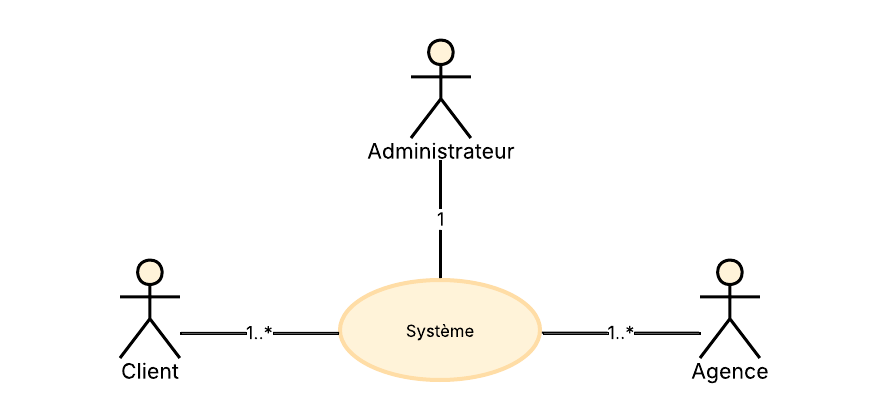
\includegraphics[width=0.7\textwidth]{Chapitres/Figures/Diag.contexte.stat.png}
    \caption{Diagramme de contexte statique}
    \label{fig:diagramme_contexte_statique}
\end{figure}

%%%%%%%%%%%%%%%%%%%%%%%%%%%%%%%%%%%%%%%%%%%%%%%%%%%%%%%%%%%%%%%%%%%%%%%%%%%
\section{Identification et analyse des besoins}
\label{section2.3}
%%%%%%%%%%%%%%%%%%%%%%%%%%%%%%%%%%%%%%%%%%%%%%%%%%%%%%%%%%%%%%%%%%%%%%%%%%%

Dans cette section, nous identifions les différentes parties prenantes du projet 
et analysons leurs besoins, qu'ils soient fonctionnels ou non fonctionnels. Cette 
étape permet de définir et d'organiser l'ensemble des exigences du système sous 
forme d'un \textbf{Product Backlog}, afin de faciliter leur gestion et leur 
priorisation pour les étapes de développement suivantes.

%%%%%%%%%%%%%%%%%%%%%%%%%%%%%%%%%%%%%%%%%%%%%%%%%%%%%%%%%%%%%%%%%%%%%%%%%%%
\subsection{Identification des besoins fonctionnels}
\label{section2.3.1}
%%%%%%%%%%%%%%%%%%%%%%%%%%%%%%%%%%%%%%%%%%%%%%%%%%%%%%%%%%%%%%%%%%%%%%%%%%%

Le besoin peut être exprimé de manière fonctionnelle, mettant en évidence les 
fonctions de services (\textit{À quoi ça sert ?}) et les fonctions techniques 
(\textit{Comment cela peut marcher ?}). Ces fonctions doivent être ordonnées, 
hiérarchisées et quantifiées sous la forme de valeurs de performance attendues.\cite{ISO}

\vspace{0.4cm}
\noindent\textbf{A. Les besoins fonctionnels de l'acteur "Internaute''}
\begin{itemize}
    \item \textbf{Consulter actualités :} L'internaute peut accéder aux informations 
    publiées sur la plateforme.
    \item \textbf{S'inscrire :} L'application permet à l'internaute de s'inscrire 
    en fournissant ses informations personnelles.
    \item \textbf{Interagir avec chatbot :} L'internaute peut poser des questions et 
    obtenir des réponses automatiques.
    \item \textbf{Contacter administrateur :} L'internaute peut envoyer un message à 
    l'administrateur pour obtenir plus d’informations .
\end{itemize}

\newpage\textbf{B. Les besoins fonctionnels de l'acteur "Utilisateur''}\\
\hspace*{0.8cm}En plus des besoins de l’acteur "Utilisateur'':
\begin{itemize}
    \item \textbf{S'authentifier :} L'utilisateur doit saisir un login et un mot de 
    passe pour accéder aux fonctionnalités de système.
    \item \textbf{Gérer profil :} L'utilisateur peut modifier ses informations 
    personnelles et ses préférences.
    \item \textbf{Consulter véhicules :} L'utilisateur peut consulter les 
    véhicules disponibles ainsi que leurs détailles.
    \item \textbf{Voir score client :} L'utilisateur peut consulter son indice de 
    fiabilité.
\end{itemize}

\textbf{C. Les besoins fonctionnels de l'acteur "Client''}\\
\hspace*{0.8cm}En plus des besoins de l’acteur "Utilisateur'':
\begin{itemize}
    \item \textbf{Effectuer réservation :} Le client peut réserver un véhicule 
    auprès d'une agence.
    \item \textbf{Consulter réservations en cours :} Le client peut suivre l'état 
    de ses réservations.
    \item \textbf{Contacter agence :} Le client peut communiquer directement avec 
    l'agence pour assistance ou négociation.
\end{itemize}

\textbf{D. Les besoins fonctionnels de l'acteur "Agence''}\\
\hspace*{0.8cm}En plus des besoins de l’acteur "Utilisateur'':
\begin{itemize}
    \item \textbf{Gérer vitrine :} L'agence peut publier et mettre à jour ses 
    véhicules disponibles.
    \item \textbf{Traiter réservations :} L'agence peut accepter ou refuser les 
    demandes de réservation ainsi que traiter les réclamations des clients..
    \item \textbf{Consulter statistiques :} L'agence peut analyser ses performances via des indicateurs.
\end{itemize}

\textbf{E. Les besoins fonctionnels de l'acteur "Administrateur''}\\
\hspace*{0.8cm}En plus des besoins de l’acteur "Utilisateur'':
\begin{itemize}
    \item \textbf{Consulter agences :} L’administrateur peut visualiser la liste des agences ainsi que leurs informations détaillées. À partir de cette interface de consultation, il peut également effectuer des actions de gestion telles que l’ajout d’une nouvelle agence, la modification des informations ou le blocage d’une agence en cas de non-conformité.
    \item \textbf{Consulter utilisateurs :} L’administrateur peut consulter les comptes la liste des utilisateurs ainsi que leurs informations. \\Depuis cette interface, il peut aussi gérer les utilisateurs en ajoutant de nouveaux comptes (en plus de l’inscription autonome), en modifiant leurs informations ou en bloquant leurs comptes si nécessaire.
    \item \textbf{Gérer messages :} L’administrateur peut consulter les messages reçus et y répondre afin d’assurer un bon suivi de la communication.
    \item \textbf{Consulter statistiques :} L’administrateur peut suivre les indicateurs de performance globaux afin de détecter les anomalies et d’améliorer le système.
\end{itemize}

%%%%%%%%%%%%%%%%%%%%%%%%%%%%%%%%%%%%%%%%%%%%%%%%%%%%%%%%%%%%%%%%%%%%%%%%%%%
\newpage
\subsection{Identification des besoins non fonctionnels}
\label{section2.3.2}
%%%%%%%%%%%%%%%%%%%%%%%%%%%%%%%%%%%%%%%%%%%%%%%%%%%%%%%%%%%%%%%%%%%%%%%%%%%

Les exigences non fonctionnelles représentent la qualité prévue de l'application et les contraintes à satisfaire lors de la réalisation des besoins fonctionnels. Notre application doit satisfaire un ensemble d'exigences non fonctionnelles :

\textbf{A. Performance}
\begin{itemize}[noitemsep, topsep=0pt]
    \item Optimiser le temps de chargement des différentes pages de l'application.
\end{itemize}
\textbf{B. Sécurité}
\begin{itemize}[noitemsep, topsep=0pt]
    \item Protéger les données personnelles des agences et des clients.
    \item Sécuriser tous les accès par authentification (login et mot de passe).
\end{itemize}
\textbf{C. Fiabilité}
\begin{itemize}[noitemsep, topsep=0pt]
    \item Garantir un fonctionnement fluide et sans erreurs critiques.
\end{itemize}
\textbf{D. Maintenabilité}
\begin{itemize}[noitemsep, topsep=0pt]
    \item Organiser le code de façon propre et structurée pour faciliter les 
    évolutions futures.
\end{itemize}
\textbf{E. Ergonomie}
\begin{itemize}[noitemsep, topsep=0pt]
    \item Offrir des interfaces intuitives, épurées et faciles à prendre en main 
    pour tous les profils d'utilisateurs.
\end{itemize}

%%%%%%%%%%%%%%%%%%%%%%%%%%%%%%%%%%%%%%%%%%%%%%%%%%%%%%%%%%%%%%%%%%%%%%%%%%%µ
\newpage
\section{Diagramme des cas d'utilisation global}
\label{section2.4}
%%%%%%%%%%%%%%%%%%%%%%%%%%%%%%%%%%%%%%%%%%%%%%%%%%%%%%%%%%%%%%%%%%%%%%%%%%%
\begin{figure}[H]
    \centering
    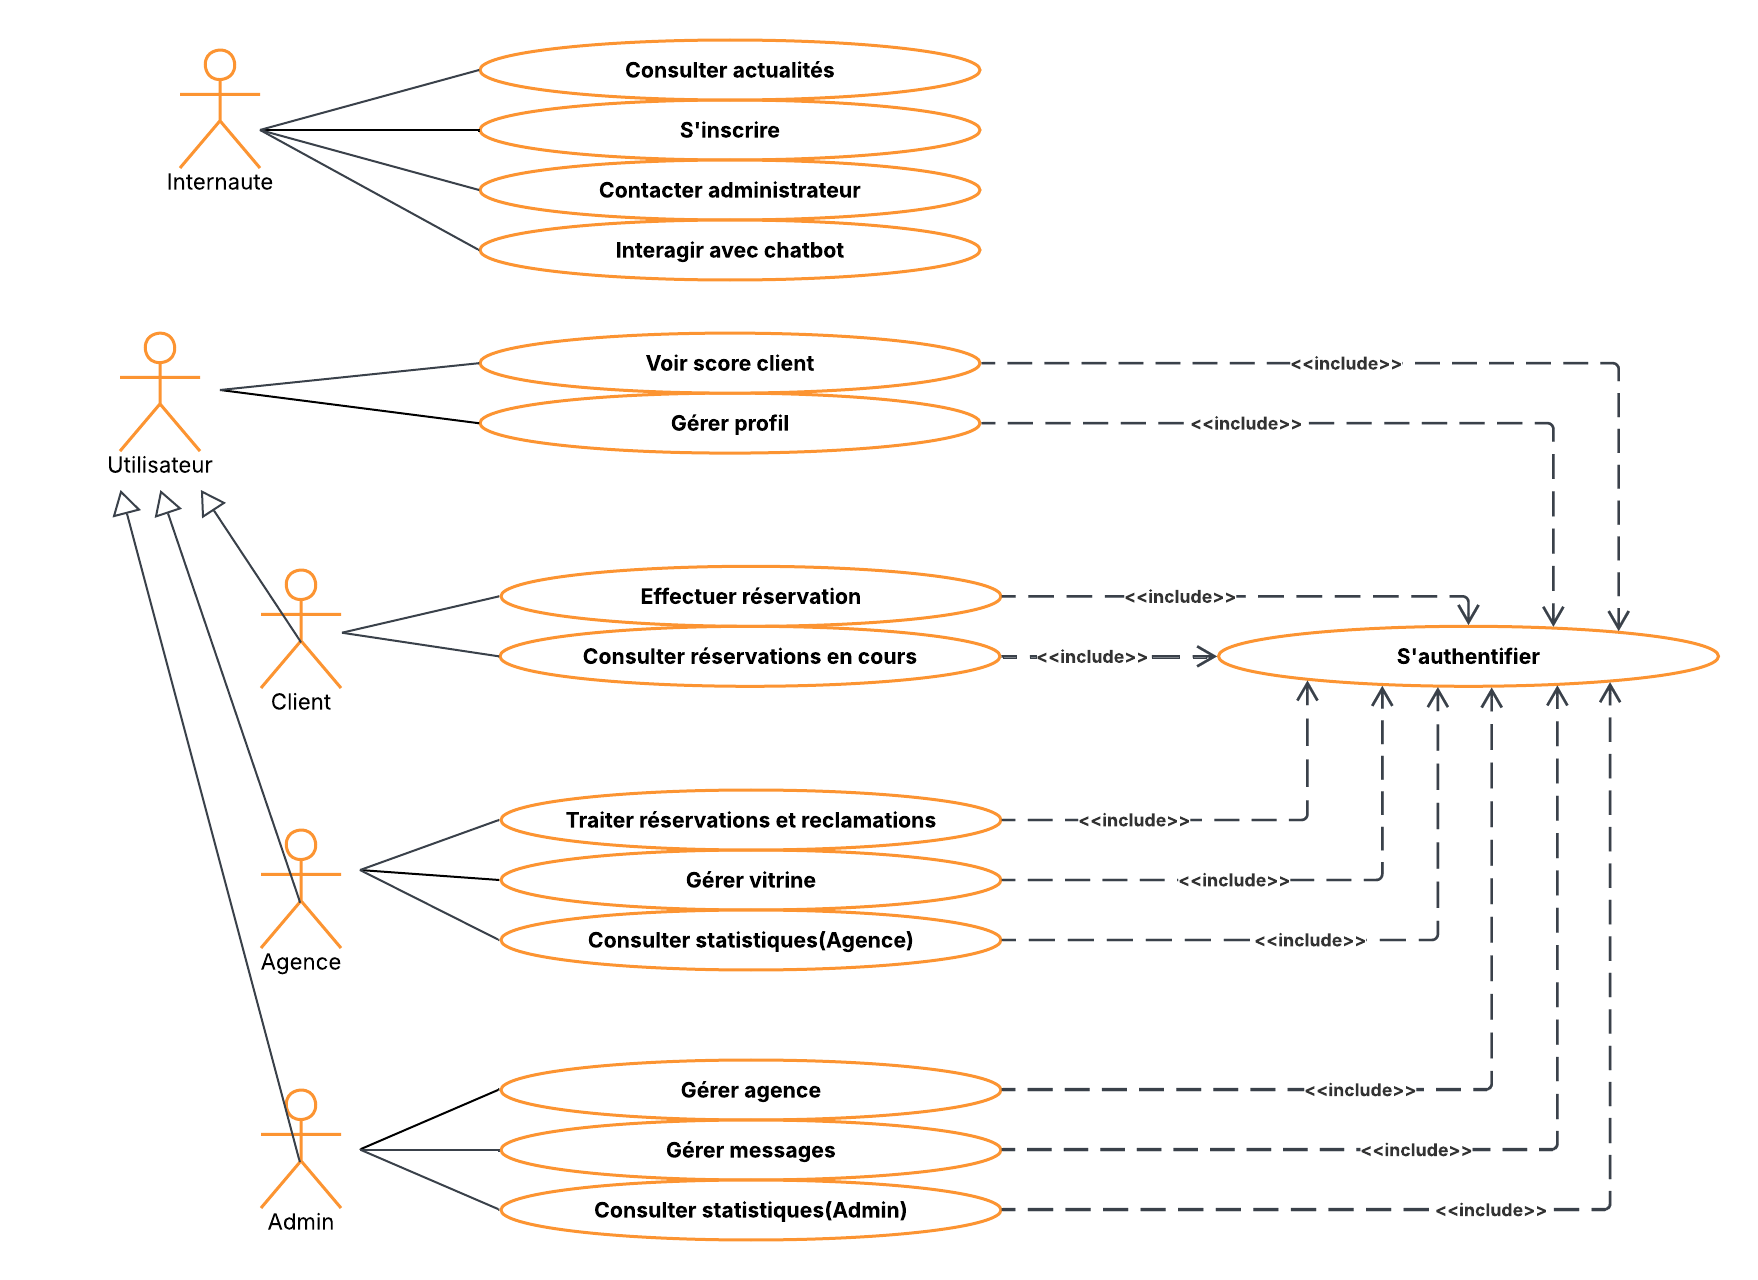
\includegraphics[width=1.2\textwidth]{Chapitres/Figures/Diag.cas.utilisation.global.png}
    \caption{Diagramme de cas d'utilisation global}
    \label{fig:cas_utilisation_global}
\end{figure}
Le diagramme de cas d'utilisation global présente une vue d'ensemble des 
interactions entre les différents acteurs (internautes, utilisateurs, clients, agences et administrateur) et notre application. Il permet de mettre en évidence les fonctionnalités principales offertes par le système ainsi que les relations hiérarchiques entre les acteurs.\cite{Lucidchart}
%%%%%%%%%%%%%%%%%%%%%%%%%%%%%%%%%%%%%%%%%%%%%%%%%%%%%%%%%%%%%%%%%%%%%%%%%%%
\newpage
\section{Identification de l'équipe Scrum}
\label{section2.5}
%%%%%%%%%%%%%%%%%%%%%%%%%%%%%%%%%%%%%%%%%%%%%%%%%%%%%%%%%%%%%%%%%%%%%%%%%%%

Dans le cadre d'une approche Scrum, il est essentiel de définir clairement les responsabilités de chaque membre de l'équipe. Les rôles Scrum structurent le travail collaboratif et garantissent une organisation efficace, assurant la transparence, la communication et l'adaptation continue tout au long du projet.

\begin{figure}[H]
    \centering
    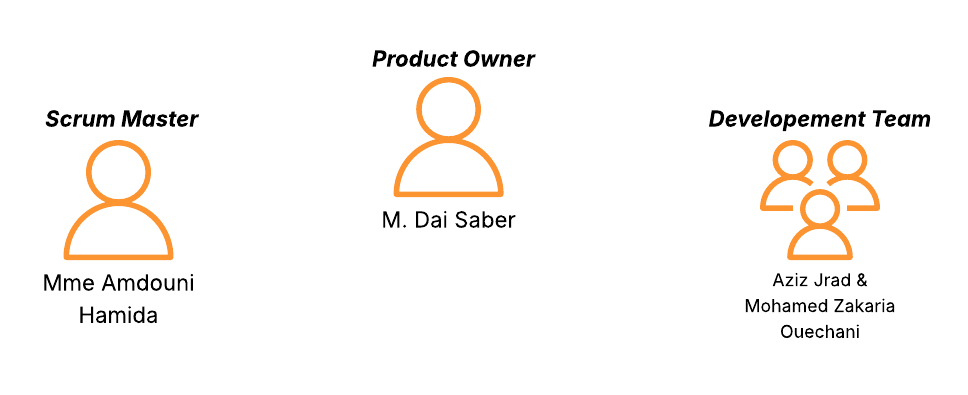
\includegraphics[width=1\textwidth]{Chapitres/Figures/Scrum-roles.png}
    \caption{Les rôles Scrum}
    \label{fig:scrum_roles}
\end{figure}

%%%%%%%%%%%%%%%%%%%%%%%%%%%%%%%%%%%%%%%%%%%%%%%%%%%%%%%%%%%%%%%%%%%%%%%%%%%
\medskip
\medskip
\medskip
\section{Le Backlog produit}
\label{section2.6}
%%%%%%%%%%%%%%%%%%%%%%%%%%%%%%%%%%%%%%%%%%%%%%%%%%%%%%%%%%%%%%%%%%%%%%%%%%%
Le \textit{Product Backlog} constitue une liste hiérarchisée de tâches qui 
définissent les caractéristiques attendues d'un produit. Il s'agit d'un élément fondamental de la méthodologie Scrum \cite{scrum}. Dans le cadre de notre projet, le backlog est structuré autour des champs suivants :
\begin{itemize}[noitemsep, topsep=3pt]
    \item \textbf{ID :} identifiant unique attribué à chaque \textit{User Story}, permettant de la distinguer et de la référencer facilement dans le backlog.
    \item \textbf{Thème :} résumé synthétique décrivant la fonctionnalité concernée, servant de regroupement logique pour plusieurs \textit{User Stories} liées.
    \item \textbf{User Story :} description du contenu fonctionnel attendu, exprimée du point de vue de l'utilisateur, sous forme de scénario simple.
    \item \textbf{Priorité :} niveau d'importance défini par le \textit{Product Owner}, indiquant l’ordre de traitement et la valeur métier associée à la fonctionnalité.
\end{itemize}

\newpage
\renewcommand{\arraystretch}{1}

\begin{longtable}{|c|c|c|p{4cm}|c|}
\caption{Backlog produit}
\label{tab:backlogproduit} \\

\hline
\textbf{Id} & \textbf{Thème} & \textbf{En tant que} & \textbf{User Story (Je veux...)} & \textbf{Priorité} \\
\hline
\endfirsthead

\hline
\textbf{Id} & \textbf{Thème} & \textbf{En tant que} & \textbf{User Story (Je veux...)} & \textbf{Priorité} \\
\hline
\endhead

\hline
\endfoot

\hline
\endlastfoot

US01 & Actualités & Internaute & consulter les actualités afin d'accéder aux informations publiées sur la plateforme & Moyenne \\ \hline
US02 & Gestion des comptes & Internaute & s'inscrire afin d'accéder aux services & Haute \\ \hline
US03 & Assistance & Internaute & interagir avec le chatbot afin d'obtenir des réponses automatiques & Moyenne \\ \hline
US04 & Support & Internaute & contacter l'administrateur afin d'obtenir plus d’informations & Haute \\ \hline
US05 & Chatbot & Internaute & interagir avec le chatbot afin d'obtenir des réponses automatiques & Moyenne \\ \hline


US06 & Authentification & Utilisateur & m'authentifier afin d'accéder aux fonctionnalités du système & Haute \\ \hline
US07 & Profil & Utilisateur & gérer mon profil afin de modifier mes informations personnelles et préférences & Moyenne \\ \hline
US08 & Véhicules & Utilisateur & consulter les véhicules disponibles ainsi que leurs détails & Haute \\ \hline
US09 & Score client & Utilisateur & voir mon score afin de connaître mon indice de fiabilité & Moyenne \\ \hline

US10 & Réservations & Client & effectuer une réservation afin de louer un véhicule auprès d'une agence & Haute \\ \hline
US11 & Réservations & Client & consulter mes réservations en cours afin de suivre leur état & Haute \\ \hline
US12 & Vitrine & Agence & gérer la vitrine afin de publier et mettre à jour les véhicules disponibles & Haute \\ \hline
US13 & Réservations & Agence & traiter les réservations afin d'accepter ou refuser les demandes et gérer les réclamations & Haute \\ \hline
US14 & Statistiques & Agence & consulter les statistiques afin d'analyser les performances & Moyenne \\ \hline

US15 & Consultation des agences & Admin & consulter les agences afin de visualiser, ajouter, modifier ou bloquer les agences & Haute \\ \hline
US16 & Consultation des utilisateurs & Admin & consulter les utilisateurs afin de visualiser, ajouter, modifier ou bloquer les comptes & Haute \\ \hline
US17 & Messages & Admin & gérer les messages afin de consulter et répondre aux utilisateurs & Moyenne \\ \hline
US18 & Statistiques globales & Admin & consulter les statistiques globales afin d'analyser les performances du système & Haute \\ \hline

\end{longtable}
%%%%%%%%%%%%%%%%%%%%%%%%%%%%%%%%%%%%%%%%%%%%%%%%%%%%%%%%%%%%%%%%%%%%%%%%%%%
\newpage
\section{La planification des sprints}
\label{section2.7}
%%%%%%%%%%%%%%%%%%%%%%%%%%%%%%%%%%%%%%%%%%%%%%%%%%%%%%%%%%%%%%%%%%%%%%%%%%%

La planification de sprint permet d'identifier les tâches qui seront accomplies pendant le sprint et la manière dont elles seront réalisées. 

\begin{figure}[H]
    \centering
    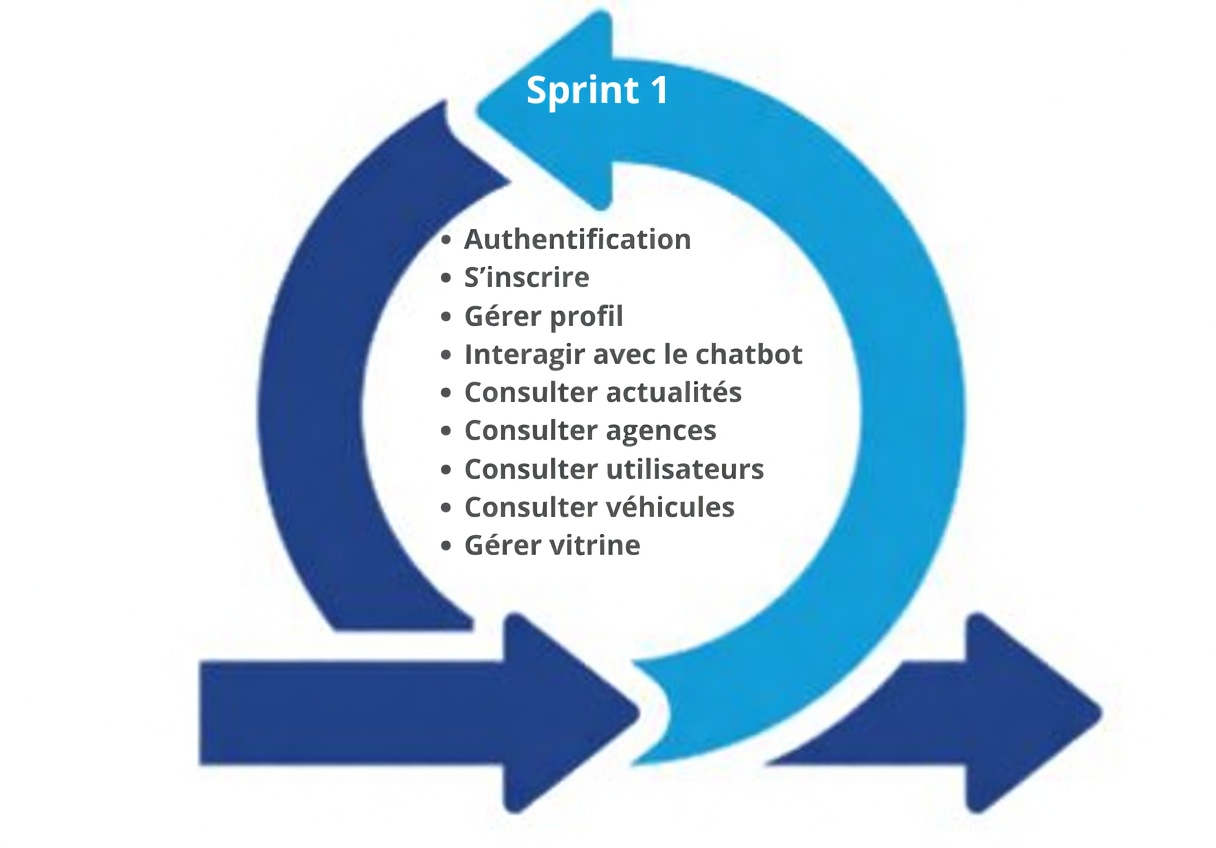
\includegraphics[width=0.7\textwidth]{Chapitres/Figures/sprint_1.png}
    \caption{Sprint 1}
    \label{fig:sprint_1}
\end{figure}
\begin{figure}[H]
    \centering
    \includegraphics[width=1\textwidth]{Chapitres/Figures/sprint_2.png}
    \caption{Sprint 2}
    \label{fig:sprint_2}
\end{figure}
%%%%%%%%%%%%%%%%%%%%%%%%%%%%%%%%%%%%%%%%%%%%%%%%%%%%%%%%%%%%%%%%%%%%%%%%%%%
\section{Diagramme de Gantt}
\label{section2.8}
%%%%%%%%%%%%%%%%%%%%%%%%%%%%%%%%%%%%%%%%%%%%%%%%%%%%%%%%%%%%%%%%%%%%%%%%%%%
Le diagramme de Gantt illustre la répartition temporelle des quatre phases du projet sur une durée totale de douze semaines.

\begin{figure}[H]
    \centering
    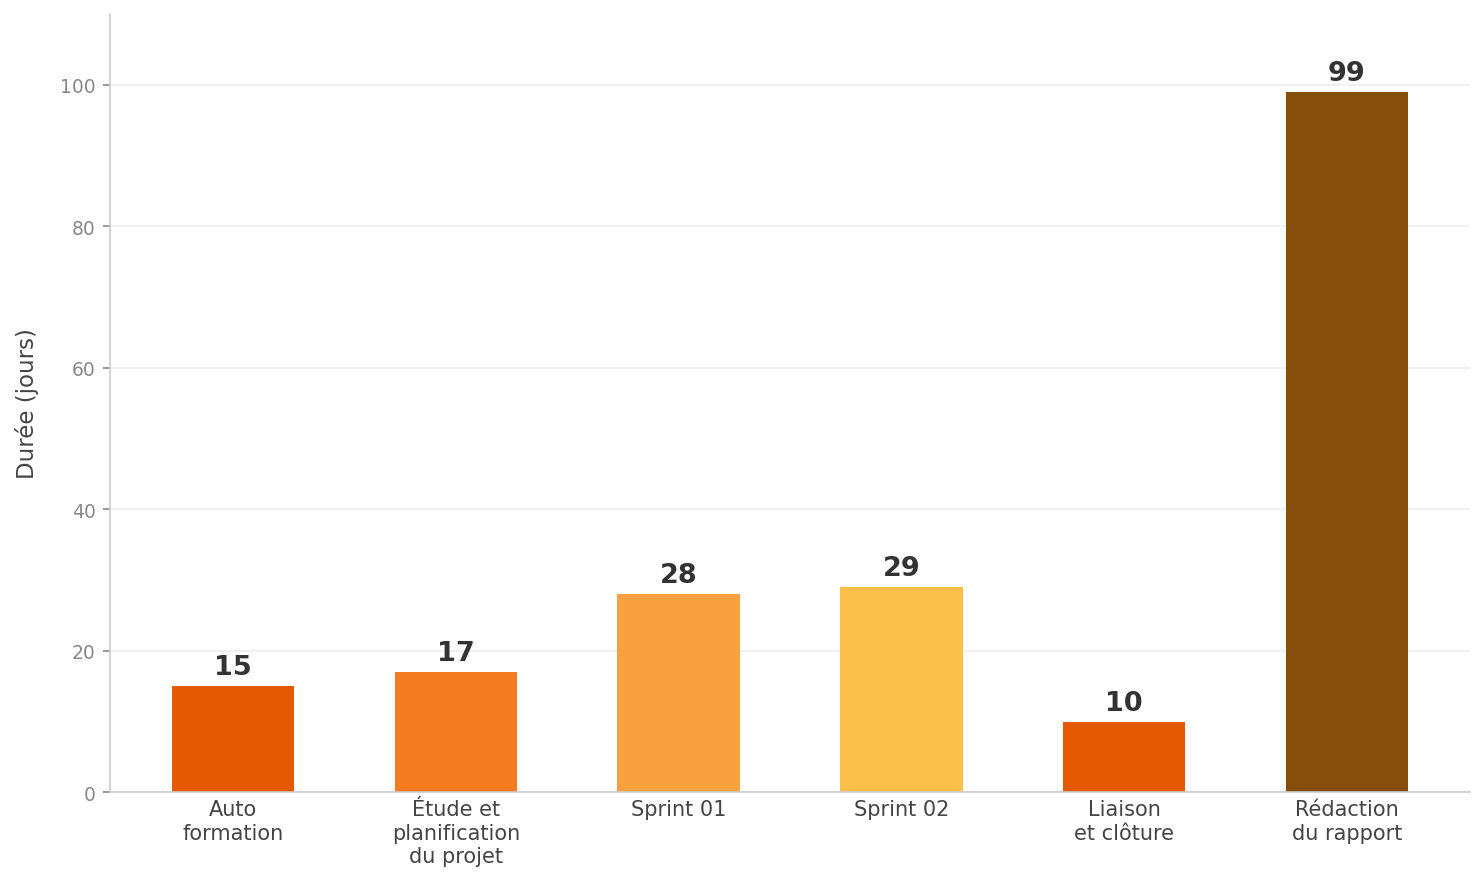
\includegraphics[width=1\textwidth]{Chapitres/Figures/gantt.png}
    \caption{Diagramme de Gantt}
    \label{fig:gantt}
\end{figure}

%%%%%%%%%%%%%%%%%%%%%%%%%%%%%%%%%%%%%%%%%%%%%%%%%%%%%%%%%%%%%%%%%%%%%%%%%%%
\section{Conclusion}
%%%%%%%%%%%%%%%%%%%%%%%%%%%%%%%%%%%%%%%%%%%%%%%%%%%%%%%%%%%%%%%%%%%%%%%%%%%

Au cours de ce chapitre, nous avons identifié les parties prenantes et défini le backlog du produit en précisant les demandes fonctionnelles et techniques de notre projet.

\medskip

Ensuite, nous avons achevé la première étape de la méthodologie Scrum en constituant l'équipe, en élaborant le diagramme global des cas d'utilisation et en établissant la liste des tâches produit ainsi que la planification des sprints.

\medskip

Le chapitre suivant sera consacré à la réalisation du \textbf{Sprint 1}, couvrant la gestion des agences, des clients et de la vitrine.